\documentclass[12pt]{article}
\usepackage{../sty/solspt}

\title{\sffamily\bfseries{Problemas Resolvidos de 13/02 - 02/03}}
\author{Samuel de Araújo Brandão}
\date{\today}

\begin{document}
\maketitle

Caro Prof. Marcelo Pena. Gostaria de iniciar esse documento pedindo perdão. A quantidade
de exercícios resolvidas é ridícula. Devo confessar que estou envergonhado com tanto desfoque e
procrastinação, resultando, assim, na baixa qualidade e quantidade das soluções. Prometo que para
as próximas semanas esforçarei-me mais para atingir muito mais conhecimento e resultados acadêmicos.

Agradeço imensamente também pela oportunidade. Me sinto extremamente honrado ao ser reconhecido
pelo senhor; admiro muito sua profissionalidade e excelência. Portanto, prometo que, equanto estiver sob
meu controle, não desapontarei o senhor. Muito pelo contrário, tenho como objetivo apresentá-lo
soluções cada vez melhores e em maior quantidade.

Se segue abaixo todas as soluções que foram escritas formalmente. Uma quantidade boa de problemas também
foram resolvidos desde nossa reunião, mas não são mencionados por não terem uma solução rigorosa escrita por mim.

\tableofcontents

\clearpage

\section{Functional Equations}
\subsection{Kyrgzstan 2012 02/13/26}
\begin{problem}
Find all functions $ f:\RR\to\RR $ such that
\[
	f(f(x)^2+f(y)) = xf(x)+y \quad \forall x,y\in \RR
\]
\end{problem}
We claim that $f(x)=\pm x$ is the only possible solution. It is clear to see that $f(x)=\pm x$ indeed works.
Now we prove it is the only two functions that actually work.

\begin{claim}
	The function $f$ is bijective.
\end{claim}
\begin{proof}
	Plugging $x=0$ gives
	\[
		f(f(0)^2+f(0))=0,
	\]
	and plugging $u=f(0)^2+f(0)$ gives $f(u)=0$. Hence, we can say $x=u$ to find that
	\[
		f(f(y))=y. \qedhere
	\]
\end{proof}
Say $f(t)=x$. Hence,
\[
	f(t^2+f(y))=f(t)\cdot t + y= f(f(t)^2+f(y)) \iff f(t)^2=t^2.
\]
However, we must still escape the pointwise trap!

By the sake of contradiction, say the function $f$ isn't one of the two linear functions we found out. Hence, say
$f(a)=+a$ and $f(b)=-b$. Thus,
\[
	f(a^2-b)=a^2+b.
\]
Contradiction! $a$ and $b$ aren't equal 0 at the same time.

\clearpage

\subsection{02/14/26}
\begin{problem}
Find all functions $f:\mathbb{R}\to\mathbb{R}$ such that
\[
	f(x^{2}+y)=f(x^{27}+2y)+f(x^{4})
\]
for all $x,y\in\mathbb{R}$.
\end{problem}
We claim the answer is $f(x)=0$. Clearly it works, so we demonstrate now that it is the only possible answer.

Say $x^2+y=x^{27}+2y$. Hence,
\[
	f(2x^2-x^{27})=f(2x^2-x^{27})+f(x^4) \iff f(x^4)=0.
\]
Thus, $f(x)=0$ for all nonnegative numbers. To prove the same is true for negative numbers and $0$,
we must simply say $y=0$, resulting in $f(x^{27})=0$.

\clearpage

\subsection{02/16/26}
\begin{problem}
Find all strictly increasing functions $f:\mathbb{Z}\to\mathbb{Z}$ such that
\[
	f(f(x))=x+2
\]
for all integers $x$.
\end{problem}
We claim the answer is $f(x)=x+1$, which clearly works. Now, we demonstrate it is the only answer.

Since $f(f(x))=x+2$,
\[
	f(f(f(x)))=f(x+2).
\]
At the same time, by saying that $f(x)=x$, we have
\[
	f(f(f(x)))=f(x)+2.
\]
Hence,
\[
	f(x+2)=f(f(f(x)))=f(x)+2.
\]

Since, $f(x)<f(x+1)<f(x+2)$ and $f: \ZZ \to \ZZ$,
\[
	f(x+1)=f(x)+1 \quad \text{and} \quad f(x)=x+f(0).
\]
Since $f(x)=x+1$ works, $f(0)=1$. Hence, the only possible answer is
\[
	f(x)=x+1.
\]

\clearpage

\subsection{02/16/26}
\begin{problem}
Find all functions $f:\mathbb{R}\to\mathbb{R}$ such that
\[
	x f(x) + y^{2} + f(xy) = f(x+y)^{2} - f(x)f(y).
\]
for all real numbers $x$ and $y$.
\end{problem}

We claim the answer is $f(x)=x$, which is clearly true. Now, we prove it is the only answer.

After replacing $x$ and $y$ and subtracting the replacements, we find
\[
	xf(x)-x^2=yf(y)-y^2 \iff g(x)=g(y).
\]
Hence, $g(x)$ is a constant $c$. Say $x=0 \iff c=0$. Hence,
\[
	xf(x)=x^2 \iff f(x)=x
\]
for every $x \neq 0$. Now, taking $x=y=0$ in the original equation, we find $f(0)=0$.

\clearpage

\section{Combinatorics}
\subsection{INMO 2020 P3}

\begin{problem}
Consider a nonempty set $S \subseteq \{0, 1, \dots, 9\}$.
It turns out that every sufficiently large positive integer
can be written as the sum of two positive integers $a$ and $b$,
where both $a$ and $b$ have decimal digits only in $S$.
How small can $|S|$ be?
\end{problem}

%% Type your solution to INMO 2020/3 (\href{https://otis.evanchen.cc/arch/20INMO3/}{20INMO3}) here ...
\begin{claim}
	$|S| \ge 5$.
\end{claim}
\begin{proof}
	AFTSOF $|S| \le 4$. Say $|S|=4$ and $S=\{p,q,r,s\}$ (making it smaller won't affect our argument).
	As defined by the statement, $a$ and $b$ have their decimal digits in $S$,
	including the ones places, that we define as $a'$ and $b'$, respectively. $a'+b' \pmod{10}$
	can result, in total, in $\binom{4}{2}+4$ different numbers: $\{0,1,2, \dots,9\}$.

	Notice that $p+p,q+q,r+r,s+s \pmod{10}$ are all different even numbers, resting only one more even inside
	$\{0,1,2, \dots,9\}$: WLOG, say it is $p+q$. Therefore, $p,q$ have the same parity, but $p,s$ and $p,r$ must
	have different parity, since we don't want more even numbers. Contradiction! In this case, $r,s$
	have the same parity, resulting in $6$ even numbers inside $\{0,1,2, \dots,9\}$, even though there are only $5$.
\end{proof}

Now, notice the following:
\begin{itemize}
	\item $0=0+0$;
	\item $1=1+0$;
	\item $2=1+1$;
	\item $3=3+0$;
	\item $4=3+1$;
	\item $5=4+1$;
	\item $6=3+3$;
	\item $7=4+3$;
	\item $8=4+4$;
	\item $9=6+3$.
\end{itemize}
Every number from $\{0,1,2,\dots,9\}$ is a result of the summation of $x,y\in S=\{0,1,3,4,6\}$.
Therefore, every number $n=a+b$, where both $a,b$ have their decimal digits $x,y\in S$.
For example: $57241$ has the following decimal digits: $\{5,7,2,4,1\}$, where
\[
	5=4+1, 7=4+3, 2=1+1, 4=3+1, 1=0+1.
\]
Hence, $57241=44130+13111$.

\begin{insight}
	Teste sua solução.
\end{insight}

\clearpage

\subsection{Soviet Union 1978}

\begin{problem}
A token is placed on an $n\times n$ chessboard.
Each of two players moves it in turn to an orthogonally neighbouring cell.
A player loses if they move the token to a cell that was already visited
(this includes the cell the token started with).
\begin{enumerate}
	\item If the token starts on a corner cell, for each $n$, who wins?
	\item If the token starts adjacent to a corner cell, for each $n$, who wins?
\end{enumerate}
\end{problem}

%% Type your solution to Soviet Union 1978 (\href{https://otis.evanchen.cc/arch/ZC1AD077/}{ZC1AD077}) here ...
\begin{enumerate}
	Call $a$ and $b$ the two players, where $a$ moves first.
	\item
	      \begin{itemize}
		      \item $n$ is an odd number. Pair every cell (except the cell where the token was initially at) with exactly one orthogonally neighbouring cell, making $2\times1$ rectangles.
		            $a$ will always move the token to a rectangle not visited by it yet, and $b$ will always be able to move the token to the other cell of this rectangle.
		            Therefore, $b$ will always be able to make a move, having this way the winning strategy.
		      \item $n$ is an even number. Pair every cell again as described above (without exceptions this time). However, now, the inverse is going to happen, since $b$ will always be the first to move the token to a
		            rectangle not visited by it before. Hence, $a$ will always be able to make a move, having this way the winning strategy.
	      \end{itemize}
	\item
	      \begin{itemize}
		      \item $n$ is an odd number. Pair every cell as described above (except the nearby corner of the initial token location).
		            Thus, we have a similar situation to the one where $n$ is an even number and the token is initially at the corner.
		            We can see that $b$ is never going to be able to go to the corner nearby the initial token's location. Hence, $a$ has the winning strategy.
		      \item $n$ is an even number. Analogous to the situation where the token is initially on a corner cell and $n$ is an even number.
		            Hence, $a$ will always be able to make a move, having this way the winning strategy.
	      \end{itemize}

\end{enumerate}
%% --------------------------------------------------
\clearpage

%%fakesubsection{Just show it's possible or impossible}

\subsection{Slovenia TST 2018}

\begin{problem}[\href{https://aops.com/community/p9543994}{Slovenia TST 2018}, $3\clubsuit$]
Let $n \ge 2$ be an integer.
There are $n^2$ marbles, each of which is one of $n$ colors,
but not necessarily $n$ of each color.
Prove that they may be placed in $n$ boxes
with $n$ marbles in each box,
such that each box contains marbles of at most two colors.
\end{problem}

%% Type your solution to Slovenia TST 2018 (\href{https://otis.evanchen.cc/arch/SVNTST/}{SVNTST}) here ...
Below we prove the statement is true for $nk$ marbles of at most $k$ colors in $k$ boxes containing $n$ marbles in each.

Clearly the statement works for the base case $k=1$. By induction over $k$, suppose the statement works for every $k$. Let's now prove it
works for $k+1$ either.

Let's divide our solution in two cases:
\begin{itemize}
	\item There are exactly $n$ marbles of each color. Hence, just fill all the boxes with $n$ marbles
	      of each color, resulting in all the boxes filled with $n$ marbles of a single color in each box.
	\item Not every color is present in exactly $n$ marbles. Let $m$ be the current number of marbles painted
	      with the less frequently used color and $M$ with the most frequently used one. Hence, we
	      might do the following algorithm:
	      \begin{enumerate}
		      \item Fill the first box with $m$. Clearly $m < n$, meaning that there is yet space to be filled in the box.
		      \item Now, take $M$ and fill the first box with $n-m$ marbles, resulting in exactly $n$ marbles in the first box of only $2$ colors.
		      \item Notice that the first box is done, so it rests now only $(k+1)-1=k$ boxes and colors to work with.
	      \end{enumerate}
\end{itemize}
Notice that the total number of marbles now is $n(k+1)-n=nk$, which satisfies the statement according to the Inductive Hypotheses.

\begin{insight}
	Inicialmente até pensei em indução, mas preciso tentar melhor provar o passo indutivo por meio da hipótese indutiva.
\end{insight}
%% --------------------------------------------------

\clearpage

\subsection{Shortlist 2012/1}

\begin{problem}
There are $n$ positive integers written in a row.
Iteratively, Alice chooses two adjacent numbers $x$ and $y$
such that $x>y$ and $x$ is to the left of $y$,
and replaces the pair $(x,y)$ by either $(y+1,x)$ or $(x-1,x)$.
Prove that she can perform at most $n^n$ such steps.
\end{problem}
Notice the maximum $M$ of the set is invariant. Take the sum
\[
	S=a_1+2a_2+\dots+na_n
\]
and say every step Alice replaces $(a_i,a_{i+1})$ by $(c,a_i)$. Hence,
every iteration results in the a difference $d$:
\[
	d=(ic+(i+1)a_i)-(ia_i+(i+1)a_{i+1})=a_i-a_{i+1}+i(c-a_{i+1}).
\]
Thus, $d \ge 1$, because $a_i > a_{i+1}$ and $c-a_{i+1} \ge 0$.

Since $S \le \frac{n(n+1)}{2}M$, it is impossible to make an infinite amount
of iterations since $S$ is up bounded, but every iteration add at least $1$ to the total sum.

\begin{insight}
	Obviamente era impossível provar sem uma soma modificada, porque sem alguma modificação válida,
	a iteração não necessariamente adicionava ou removia algo da soma total. Logo, imediatamente
	poderia se imaginar em mudar isso.
\end{insight}

\clearpage

\section{Geometry}
\subsection{Iran TST 2011/1 02/13/2026}
\begin{problem}
In acute triangle $ABC$, $\angle B>\angle C$.
Let $M$ be the midpoint of $\overline{BC}$ and let $E$ and $F$ be the feet of the altitudes from $B$ and $C$, respectively.
Let $K$ and $L$ be the midpoints of $\overline{ME}$ and $\overline{MF}$, respectively, and let $T$ lie on line $KL$ such that $\overline{TA}\parallel \overline{BC}$.
Prove that $TA=TM$.
\end{problem}
\begin{figure}[h]
	\centering
	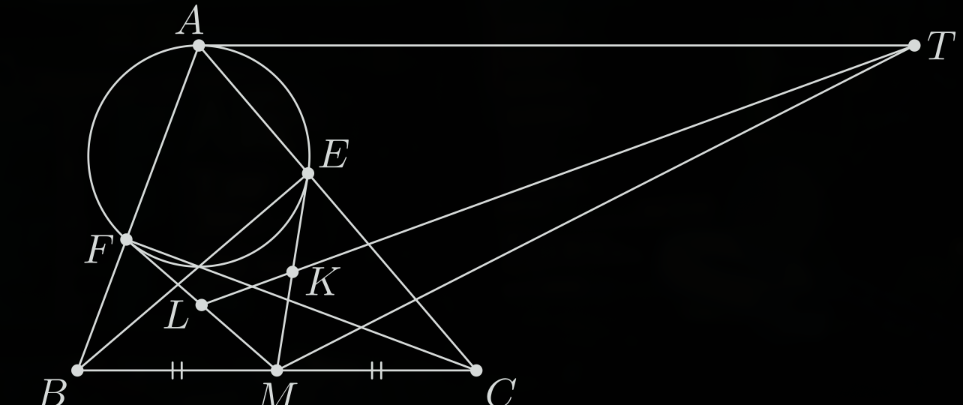
\includegraphics[width=0.6\textwidth]{geo/img/sols/iran}
\end{figure}
Let $\Gamma_1=(AFE)$ and $\Gamma_2$ be the circumference of radius $0$  centered at $M$. In order to prove $TA=TM$, it is enough to demonstrate that $\operatorname{Pow}_{\Gamma_1}(T)=\operatorname{Pow}_{\Gamma_2}(T)$.
\begin{claim}
	$\overline{KL}$ is the radical axis of $\Gamma_1$ and $\Gamma_2$.
\end{claim}
\begin{proof}
	By the Three Tangents Lemma, $\overline{ME}$ and $\overline{MF}$ are both tangents to $\Gamma_1$. Since, $MK=KE$,
	\[
		\operatorname{Pow}_{\Gamma_1}(K)=\operatorname{Pow}_{\Gamma_2}(K).
	\]
	Hence,
	$K$ lies inside the radical axis of $\Gamma_1$ and $\Gamma_2$. However, we can use an analogous argument to prove that $L$ does either. Hence $\overline{KL}$ is the radical axis of $\Gamma_1$ and $\Gamma_2$.
\end{proof}
Since $K$, $L$ and $M$ are collinear, $M$ lies inside this radical axis too. Hence, $TA=TM$

\clearpage

\subsection{02/13/26}
\begin{problem}
Let $\overline{AD}$, $\overline{BE}$, $\overline{CF}$ be the altitudes of a scalene triangle $ABC$ with circumcenter $O$. Prove that $(AOD)$, $(BOE)$, and $(COF)$ intersect at point $X$ other than $O$.
\end{problem}
\begin{figure}[h]
	\centering
	
\includegraphics[width=0.6\textwidth]{geo/img/sols/1.png}
\end{figure}
Let $H$ be the orthocenter $\triangle ABC$. Hence,
\[
	HA \cdot HD = HB \cdot BE = HC \cdot HF,
\]
is true by considering the circumcenters of diameters $AB$, $BC$ and $CA$.
Which means that both $O$ and $H$ have the same power of point of all the circumferences $(AOD)$, $(BOE)$, and $(COF)$.

Hence, those three circumferences have the same radical axis, resulting in another point $X$ where they three intersect.

\clearpage

\section{Number Theory}
\subsection{1.12.3}
\begin{problem}
Let $x,y,a,b,c$ be integers.
\begin{enumerate}
	\item Prove that $2x+3y$ is divisible by $17$ if and only if $9x+5y$ is divisible by $17$.
	\item If $4a+5b-3c$ is divisible by $19$, prove that $6a-2b+5c$ is also divisible by $19$.
\end{enumerate}
\end{problem}
\begin{enumerate}
	\item Say
	      \[
		      17 \mid 2x+3y \iff 17 \mid k(2x+3y).
	      \]
	      However, $k(2x+3y)-9x-5y=x(2k-9)+y(3k-5)$. Notice that $k=13$ results in $17x+34y$, which is
	      a multiple of $17$. Thus, if $2x+3y$ is divisible by $17$, $9x+5y$ is either. An analogous
	      solution proves the if and only if.
	\item Analogous argument proves the statement.
\end{enumerate}

\clearpage

\subsection{1.12.4}
\begin{problem}
Define the $n$th Fermat number $F_n$ by $F_n=2^{2^n}+1$. Show that $F_m,F_n$ are coprime for any $m,n$
\end{problem}
\begin{claim}
	$(2^{2^{m}}+1) \equiv 2 \pmod{(2^{2^{n}}+1)} \quad \forall m>n$.
\end{claim}
\begin{proof}
	Let $a=2^{2^{n}}$. Hence, we must prove
	\[
		a+1 \mid 2^{2^{m}}-1.
	\]
	Notice $2^{2^{m}}=(2^{2^{n}})^{2^{m-n}}=a^{2^{m-n}}$. Since $m<n$, say $a^{2^{m-n}}=2t$. Therefore, it suffices to prove that
	\[
		a+1 \mid a^{2^{m-n}}-1 = a^{2t}-1=(a+1)(a^{2t-1}+a^{2t-2}-\dots+1) \qedhere
	\]
\end{proof}
Therefore, $F_m$ and $F_n$ are clearly coprime.

\end{document}
